\section{Chapter problems}
\subsection{Chapter 1}
\paragraph{Problem 1}
Suppose the universal set is defined as $S=\{x\in \mathbb{N} | 1\geq x \geq 10\}$, $A=\{1,2,3\}$, $B=\{x\in S|2\geq x\geq 7\}$ and $C=\{7,8,9,10\}$.

a) Find $A\cup B$
\[
    A\cup B=\{1,2,3\}\cup\{2,3,4,5,6,7\}=\{1,2,3,4,5,6,7\}
\]
b) Find $(A\cup C)\setminus B$
\[
    (A\cup C)\setminus B=\{1,2,3,7,8,9,10\}\setminus \{2,3,4,5,6,7\}=\{1,8,9,10\}
\]
c) Find $\overline{A}\cup(B\setminus C)$
\[
    \overline{A}\cup(B\setminus C)=\{4,5,6,7,8,9,10\}\cup\{2,3,4,5,6\}=\{2,3,4,5,6,7,8,9,10\}
\]
d) Do $A,B$ and $C$ form a partition of $S$?

No as $A\cap B\neq\emptyset$ and $B\cap C\neq\emptyset$.
\paragraph{Problem 2}
When working with real numbers, our universal set is $\mathbb{R}$. Find each of the following sets
a) $[6,8]\cup[2,7[$
\[
    [2,8]
\]
b) $[6,8]\cap[2,7[$
\[
    [6,7[
\]
c) $\overline{[0,1]}$
\[
    ]-\infty,0[\cup]1,\infty[
\]
d) $[6,8]\setminus ]2,7[$
\[
    [7,8]
\]
\paragraph{Problem 3}
For each of the follopwing Venn diagrams, write the sets denoted by the shaded area

a)
\[
    A\cup B\setminus A\cap B
\]
b)
\[
    B\setminus C
\]
c)
\[
    A\cap B+A\cap C
\]
d)
\[
    C\cup(A\cap B)\setminus ((C\cap A)\cup (C\cap B))
\]
\paragraph{Problem 4}
A coin is tossed twice. Let $S=\{H,T\}\times\{H,T\}$. Write the following sets by listing their elements:

a) First toss is heads
\[
    A=\{(H,T),(H,H)\}
\]
b) At least one tails
\[
    B=\{(T,T),(T,H),(H,T)\}
\]
c) Two tosses are different
\[
    C=\{(H,T),(T,H)\}
\]
\paragraph{Problem 5}
Let $A=\{1,2,\ldots,100\}$. For any $i\in \mathbb{N}$, define $A_{i}$ as the set of numbers in $A$ that are divisible by $i$.

a)
\begin{align*}
    |A_{1}|&=\left\lfloor{\frac{|S|}{1}}\right\rfloor=\left\lfloor{\frac{100}{1}}\right\rfloor=100 \\
    |A_{2}|&=\left\lfloor{\frac{|S|}{2}}\right\rfloor=\left\lfloor{\frac{100}{2}}\right\rfloor=50 \\
    |A_{3}|&=\left\lfloor{\frac{|S|}{3}}\right\rfloor=\left\lfloor{\frac{100}{3}}\right\rfloor=33 \\
    |A_{4}|&=\left\lfloor{\frac{|S|}{4}}\right\rfloor=\left\lfloor{\frac{100}{4}}\right\rfloor=25 \\
    |A_{5}|&=\left\lfloor{\frac{|S|}{5}}\right\rfloor=\left\lfloor{\frac{100}{5}}\right\rfloor=20
\end{align*}
b)

By the distributive property we have that
\[
    A_2\cap A_3\cap A_5=(A_2\cap A_3)\cap A_5
\]
As the intersection of $A_2$ and $A_3$ must be the even factors of 3 we get
\[
    A_2\cap A_3=\{x\in A|x=6n,n\in \mathbb{N}\}
\]
The cardinality of this must be half of the original as every other value is valid
\[
    |A_2\cap A_3|=\left\lfloor{\frac{33}{2}}\right\rfloor=16
\]
As only every fifth factor of 6 is a factor of 5 we get that
\[
    A_2\cap A_3\cap A_5=\{x\in A|x=30n,n\in \mathbb{N}\}
\]
As this is every fifth value of the previous intersection, the cardinality must be one fifth of the previous
\[
    |A_2\cap A_3\cap A_5|=\left\lfloor{\frac{16}{5}}\right\rfloor=3
\]

\paragraph{Problem 6}
As $A_1,A_2,A_3$ form a partition of the universal set, the cardinality of $B$ must be equal to the sum of the cardinalities in the individual partitions.
\[
    |B|=\sum_{i=1}^{3} |B\cap A_i|=10+20+15=45
\]
\paragraph{Problem 7}
a)
As the numbers can be listed in one-to-one correspondance with the natural numbers the set is countable.

b) As the set is made up of the union of 2 countable sets we have that
\[
    B=\bigcup_{i=\mathbb{Q}}\bigcup_{j=\mathbb{Q}}\{a_i+b_j\sqrt{2}\}
\]
As such it must be countable as its constituents are.

c) As the set is a subset of an uncountable set (real numbers), it is not countable.

\paragraph{Problem 8}
We take the limit of the upper bound of the interval as $n\rightarrow\infty$
\[
    \lim_{n\rightarrow\infty}\frac{n-1}{n}=1
\]
As this limit is the upper bound of the interval, corresponding to the maximal interval included in the union of sets we get that
\[
    A=\bigcup_{n=1}^{\infty}A_n=[0;1[
\]
\paragraph{Problem 9}
Opposed to the previous problem the smallest set will here define the set as the intersection is limited to the smallest component. We take the limit as $n\rightarrow \infty$ as the value is inverse proportional to $n$
\[
    \lim_{n\rightarrow\infty}\frac{1}{n}=0
\]
As such
\[
    A=\bigcap_{n=1}^{\infty}A_n=\{0\}
\]
\paragraph{Problem 10}
a)


b)


\paragraph{Problem 11}
As the set is given as an interval it is clear that
\[
    [0,1[\subset\mathbb{R}
\]
As subsets of uncountable sets are uncountable, it becomes clear that the range is uncountable.
\paragraph{Problem 12}
a)

Reading the function it becomes clear that the domain of the function is given by
\[
    \{H,T\}^{3}
\]
While the co-domain is given by
\[
    \mathbb{N}\cup \{0\}
\]
b)

As the function is limited by the amount of heads that can appear in the sequence it is clear that
\[
    \text{Range}(f)=\{0,1,2,3\}
\]
c)

Knowing that $x=2$ tells us that 2 heads are present in the sequence, and as such 1 tails must also be present, as such the possible events are
\[
    \{(H,H,T),(H,T,H),(T,H,H)\}
\]
\paragraph{Problem 13}
a)

We logically assume that the events are disjoint as two teams cant win, as such it is clear that
\[
    0.5+P(b)+0.25=1\Leftrightarrow P(b)=1-0.5-0.25=0.25
\]
b)
As the events are disjoint we determine the probability as
\[
    P(b\cup d)=0.25+0.25=0.5
\]
\paragraph{Problem 14}
a)

By inclusion-exclusion principle we have that
\[
    P(A\cap B)=P(A)+P(B)-P(A\cup B)=0.4+0.7-0.9=0.2
\]
b)

We have that
\[
    P(\overline{A}\cap B)=P(B\setminus A)
\]
Expanding this expression we get that
\[
    P(\overline{A}\cap B)=P(B)-P(A\cap B)=0.7-0.2=0.5
\]
c)

Expanding the expression we again get
\[
    P(A\setminus B)=P(A)-P(A\cap B)=0.4-0.2=0.2
\]
d)

Expanding the expression we get
\[
    P(\overline{A}\setminus B)=P(\overline{A})-P(\overline{A}\cap B)=(1-0.4)-0.5=0.1
\]
e)

By the inclusion-exclusion principle we have
\[
    P(\overline{A}\cup B)=P(\overline{A})+P(B)-P(\overline{A}\cap B)=(1-0.4)+0.7-0.5=0.8
\]
f)
By the distributive law
\[
    A\cap(B\cup\overline{A})=(A\cap B)\cup(A\cap \overline{A})
\]
As
\[
    A\cap\overline{A}=\emptyset
\]
by definition. We get that
\[
    P(A\cap(B\cup\overline{A}))=P((A\cap B)\cup\emptyset)=0.2
\]
\paragraph{Problem 15}
a)

We assume the rolls are independent, as such
\[
    P(X_2=4)=\frac{1}{6}
\]
b)

The sample space is given by
\begin{equation*}
  \begin{gathered}
      S=\{(1,1),(1,2),(1,3),(1,4),(1,5),(1,6),(2,1),(2,2),(2,3),(2,4), \\
      (2,5),(2,6),(3,1),(3,2),(3,3),(3,4),(3,5),(3,6),(4,1),(4,2), \\
      (4,3),(4,4),(4,5),(4,6),(5,1),(5,2),(5,3),(5,4),(5,5), \\
      (5,6),(6,1),(6,2),(6,3),(6,4),(6,5),(6,6)\}$
  \end{gathered}
\end{equation*}
The outcomes that satisfy the event are
\[
    \{X_1+X_2=7\}=\{(1,6),(2,5),(3,4),(4,3),(5,2),(6,1)\}
\]
As such
\[
    P(X_1+X_2=7)=\frac{6}{36}=\frac{1}{6}
\]
c)

As they are independent we determine the probability as
\[
    P(X_1\neq 2\cap X_2\geq 4)=P(X_1\neq 2)P(X_2\geq 4)=\frac{5}{6}\cdot\frac{3}{6}=\frac{15}{36}=\frac{5}{12}
\]
\paragraph{Problem 16}
a)

As the sum of the individual probabilities must equate to 1 we wish to determine a $c$ that satisfies the equation
\[
    \sum_{k=1}^{\infty}P(k)=\sum_{k=1}^{\infty}\frac{c}{3^{k}}=1
\]
We apply the formula for a geometric series
\[
    \sum_{k=0}^{\infty}cr^{k}=\frac{a}{1-r}\text{ for }|r|<1
\]
As this starts from $0$ we subtract $c$ as $P(\{0\}])=\frac{c}{k^{0}}=c$
\begin{align*}
    1&=-c+\sum_{k=0}^{\infty}c\left(\frac{1}{3}\right)^{k} \\
     &=-c+\frac{c}{1-\frac{1}{3}}
\end{align*}
By isolation for $c$ we then get that
\[
    \frac{2}{3}=-\frac{2}{3}c+c\Leftrightarrow \frac{2}{3}=\frac{1}{3}c\Leftrightarrow 2=c
\]
b)

The set is given by the union of the 3, as such
\begin{align*}
    P(\{2,4,6\})&=P(\{2\}\cup \{4\}\cup \{6\}) \\
              &=P(\{2\})+P(\{4\})+P(\{6\}) \\
              &=\frac{2}{9}+\frac{2}{81}+\frac{2}{729} \\
              &=\frac{182}{729}
\end{align*}
c) This must equate to the complement of $P(\{1,2\})$, as such
\begin{align*}
    P(\{3,4,5,\ldots\})&=1-P(\{1,2\}) \\
              &=1-\left(\frac{2}{3}+\frac{2}{9}\right) \\
              &=1-\frac{8}{9} \\
              &=\frac{1}{9}
\end{align*}
\paragraph{Problem 17}
We have that
\begin{align*}
    P(A)&=P(B) \\
    P(C)&=2P(D) \\
    P(A\cup C)&=P(A)+P(C)=0.6
\end{align*}
We rewrite all terms as functions of $P(A)$, these must equate to 1 as a team has to win, making it the sample space
\begin{align*}
    1&=P(A)+P(A)+(0.6-P(A))+\frac{0.6-P(A)}{2} \\
     &=0.5P(A)+0.9
\end{align*}
Isolating for $P(A)$ we get
\[
    P(A)=\frac{1-0.9}{0.5}=0.2
\]
From this we can determine the rest of the probabilities using the requirements set earlier
\begin{align*}
    P(A)&=P(B)=0.2 \\
    P(C)&=0.6-P(A)=0.4 \\
    P(D)&=0.5P(C)=0.2 \\
    \sum P&=0.2+0.2+0.4+0.2=1
\end{align*}
\paragraph{Problem 18}
a)

We insert $t=1$
\[
    P(T\leq 1)=\frac{1}{16}1^{2}=\frac{1}{16}
\]

b) 

This must equate to the complement of it taking 2 hours, as such
\[
    P(2>t)=1-\left(\frac{1}{16}2^{2}\right)=\frac{3}{4}
\]
c)

This equates to the difference between the probability of the job taking more than 1 hour and more than 3 hours
\[
    P(1\leq T\leq 3)=P(T\leq 1)-P(T\leq 3)=\frac{1}{16}3^{2}-\frac{1}{16}1^{2}=\frac{1}{2}
\]
\paragraph{Problem 19}
The problem has the form of the quadratic equation
\[
    ax^{2}+bx+c=0\implies x=\frac{-b\pm\sqrt{b^{2}-4ac}}{2a}
\]
For this to have real solutions it is necessary that
\[
    b^{2}-4ac\geq 0\vee a\neq 0
\]
Translating this to the given equation we wish to determine values $A,B\in[0,1]$ that satisfy
\[
    1^{2}-4AB\geq 0\vee A\neq 0
\]
Seeing this as a function based on the given figure, we write that
\[
    1^{2}-4xy\geq 0
\]
Isolating for $y$ it becomes apparent that
\begin{align*}
    1^{2}-4xy&\geq 0 \\
    1^{2}&\geq 4xy \\
    \frac{1}{4x}&\geq y
\end{align*}
As the maximal $y$-value is 1 we determine the intersection
\[
    1=\frac{1}{4x}\Leftrightarrow x=\frac{1}{4}
\]
Now we can determine the probability as the proportion of the area that fits under this curve in the interval for which it is inside the unit square
\begin{align*}
    P(1-4AB\geq 0)&=\frac{1}{4}+\frac{1}{4}\int_{\frac{1}{4}}^{1}\frac{1}{4x} \\
               &=\frac{1}{4}+\frac{1}{4}\left[\ln{x}\right]_{\frac{1}{4}}^{1} \\
               &=\frac{1}{4}+\frac{1}{4}\left(\ln{1}-\ln{\frac{1}{4}}\right) \\
               &\approx\frac{3}{5}
\end{align*}
\paragraph{Problem 20}
a) 

As every set is a subset of the next, it is clear that $A_n$ will be the largest or equal to the largest set in the sequence, as such
\[
    P\left(\bigcup_{i=1}^{\infty}A_i\right)=\lim_{n\rightarrow \infty}P(A_n)
\]
As all the sets are subsets of $A_n$ and therefore their union will create $A_n$.

b)

Here it is the opposite where $A_n$ will be the smallest or equal to the smallest set in the sequence as such
\[
    P\left(\bigcap_{i=1}^{\infty} A_i\right)=\lim_{n\rightarrow\infty} P(A_n)
\]
As the intersection will always be limited by the smallest set in the sequence.

\paragraph{Problem 21 DO LATER}
\paragraph{Problem 22}
Let $A$ be the event that the customer purchased a cup of coffee and $B$ the event they purchased a piece of cake, then
\begin{align*}
    P(A)&=0.7 \\
    P(B)&=0.4 \\
    P(A\cap B)&=0.2
\end{align*}
By conditional probability we have that
\begin{align*}
    P(A|B)&=\frac{P(A\cap B)}{P(B)} \\
          &=\frac{0.2}{0.4} \\
          &=0.5
\end{align*}
\paragraph{Problem 23}
a)
\begin{align*}
    P(A|B)&=\frac{P(A\cap B)}{P(B)} \\
          &=\frac{0.2}{0.35} \\
          &\approx 0.57
\end{align*}
b)
\begin{align*}
    P(C|B)&=\frac{P(B\cap C)}{P(B)} \\
          &=\frac{0.15}{0.35} \\
          &\approx0.43
\end{align*}
c)
\begin{align*}
    P(B|A\cup C)&=\frac{P(B\cap(A\cup C))}{P(A\cup C)} \\
          &=\frac{0.25}{0.7} \\
          &\approx 0.36
\end{align*}
d)
\begin{align*}
    P(B|A\cap C)&=\frac{P(B\cap(A\cap C))}{P(A\cap C)} \\
          &=\frac{0.1}{0.2} \\
          &=0.5
\end{align*}
\paragraph{Problem 24}
As this is an interval with infinite points, we determine the proportion of the interval that is spanned by the interval were observing, as such
\[
    P(A\leq X\leq B)=\frac{B-A}{10}
\]
a)
\[
    P(2\leq X\leq 5)=\frac{5-2}{10}=0.3
\]
b)
\[
    P(X\leq 2|X\leq 5)=\frac{2}{5}=0.4
\]
c)
\begin{align*}
    P(3\leq X\leq 8|X\geq 4)&=\frac{P(3\leq X\leq 8\cap X\geq 4)}{X\geq 4} \\
                   &=\frac{P(4\leq X\leq 8)}{0.6} \\
                   &=\frac{\frac{8-4}{10}}{0.6} \\
                   &=\frac{2}{3}
\end{align*}
\paragraph{Problem 25}
We define the event $A$ as getting an A in the course and $B$ as living on campus
\begin{align*}
    P(A)&=\frac{120}{600}=0.2 \\
    P(B)&=\frac{200}{600}=\frac{1}{3} \\
    P(A|\overline{B})&=\frac{80}{400}=0.2
    P(A|B)&=\frac{40}{200}=0.2
\end{align*}
For $A$ and $B$ to be independent we would expect
\[
    P(A|B)=P(A)
\]
Which is true, as such, the 2 events are independent.
\paragraph{Problem 26}
Define $N_1,N_6$ as the number of times out of $n$ that a 1 or 6 is rolled, and let $X_i$ be the $i$'th roll, then
\[
    P(N_1\geq 1\cap N_6\geq 1)=1-P(\overline{N_1\geq 1\cap N_6\geq 1})
\]
By De Morgans Law we get
\begin{align*}
    &=1-P(N_1=0\cap N_6=0) \\
    &=1-(P(X_1\neq 1,X_2\neq 1,\ldots,X_n\neq 1)+P(X_1\neq 6,X_2\neq 6,\ldots,X_n\neq 6) \\ 
    &-P((X_1\neq 1,X_2\neq 1,\ldots,X_n\neq 1)\cap (X_1\neq 1, X_2\neq 6,\ldots, X_n\neq 6))) 
\end{align*}
As the final term is equivalent to
\[
    \bigcap_{i=1}^{n} P(X_{i}\neq 1\cap X_{i}\neq 6)
\]
We get that
\begin{align*}
    &=1-\left(2\left(\frac{5}{6}\right)^{n}-\left(\frac{4}{6}\right)^{n}\right) \\
    &=1-\frac{2\cdot5^{n}-4^{n}}{6^{n}}
\end{align*}
\paragraph{Problem 27}
a)

Tree is finished on paper.

b) 

We sum the probabilities that result in an error
\begin{align*}
    P(E)&=P(E|G)+P(E\overline{G}) \\
        &=0.08+0.06 \\
        &=0.14
\end{align*}

c)

From the definition of conditional probability we have
\begin{align*}
    P(G|\overline{E})&=\frac{P(G\cap\overline{E})}{P(\overline{E})} \\
                     &=\frac{0.72}{1-0.14} \\
                     &=\frac{0.72}{0.86} \\
                     &\approx 0.84
\end{align*}
\paragraph{Problem 28}
We define $D$ as the unit being defective, the probability of picking a defective unit on the first draw is
\[
    P(D_1)=\frac{5}{100}
\]
Assuming that one wasnt defective the next draw has
\[
    P(D_2|\overline{D_1})=\frac{5}{99}
\]
And the 3rd
\[
    P(D_3|\overline{D_2},\overline{D_1})=\frac{5}{98}
\]
We wish to determine the probaility of the event
\[
    P(D=1)=P(\{(D,\overline{D},\overline{D}),(\overline{D},D,\overline{D}),(\overline{D},\overline{D},D)\})
\]
As these are disjoint we determine them as the sum of their individual probailities
\begin{align*}
P(D=1)&=P(\{(D,\overline{D},\overline{D})\})+P(\{\overline{D},D,\overline{D}\})+P(\{\overline{D},\overline{D},D)\}) \\
      &=\frac{5}{100}\cdot\frac{95}{99}\cdot\frac{94}{98}+\frac{95}{100}\cdot\frac{5}{99}\cdot\frac{94}{98}+\frac{95}{100}\cdot\frac{94}{99}\cdot\frac{5}{98} \\
      &\approx 0.14
\end{align*}
\paragraph{Problem 29}
a)

As the components are connected in series, the probability of the system being functional is equal to the complement of one or more of the components not working. Let $F$ be the event that the system is functional and $P(C_i)$ be the event that the $i$'th component is functional.
\[
    P(F)=P(C_1\cap C_2\cap C_3)=P(C_1)P(C_2)P(C_3)
\]
b)

As they're connected in parallel they must all fail for the circuit to be non-functional, as such the probability must be given be the union of them
\[
    P(F)=P(C_1\cup C_2\cup C_3)
\]
By the inclusion-exclusion principle
\begin{equation*}
    \begin{gathered}
        P(F)=P(C_1)+P(C_2)+P(C_3)-P(C_1)P(C_2)-P(C_1)P(C_3)- \\
        P(C_2)P(C_3)+P(C_1)P(C_2)P(C_3)
    \end{gathered}
\end{equation*}

c)

The probability that this circuit works must be given by the probability that either $C_1$ and $C_3$ or $C_2$ and $C_3$ are functional.
\begin{align*}
    P(F)&=P((C_1\cap C_3)\cup(C_2\cap C_3)) \\
        &=P(C_1\cap C_3)+P(C_2\cap C_3)-P((C_1\cap C_3)\cap(C_2\cap C_3)) \\
        &=P(C_1)P(C_3)+P(C_2)P(C_3)-P(C_1\cap C_2\cap C_3)
\end{align*}

d)

The probability that this circuit works is given by the probability that either $C_3$ or both $C_1$ and $C_2$ work
\begin{align*}
    P(F)&=P(C_3\cup(C_1\cap C_2)) \\
        &=P(C_3)+P(C_1\cap C_2) \\
        &=P(C_3)+P(C_1)P(C_2)-P(C_1)P(C_2)P(C_3)
\end{align*}
e)

The probability that this circuit works is determined by whether $C_1,C_2$ and $C_5$ or $C_3,C_4$ and $C_5$ work, therefore
\begin{align*}
    P(F)&=P(C_1\cap C_2\cap C_5)+P(C_3\cap C_4\cap C_5)-P(C_1\cap C_2\cap C_3\cap C_4\cap C_5) \\
        &=P(C_1)P(C_2)P(C_5)+P(C_3)P(C_4)P(C_5)-\prod_{i=1}^{5}P(C_i)
\end{align*}
\paragraph{Problem 30}
a) 

Rewriting the set as a piecewise function we get
\[
    A=\begin{cases}
        x-y\leq \frac{1}{2} & x\geq y \\
        y-x\leq\frac{1}{2} & y\geq x
    \end{cases}
    \implies
    \begin{cases}
        y\leq x-\frac{1}{2} & x\geq y \\
        y\leq \frac{1}{2}+x & y\geq x
    \end{cases}
\]
At the same time $B$ is equal to the area above the $45\degree$ line in the unit square. Drawing this in Geogebra gives us

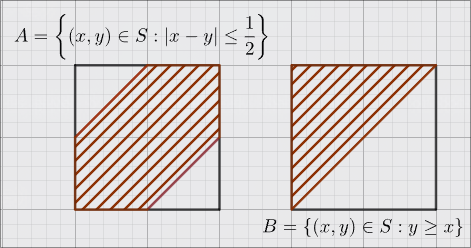
\includegraphics[width=\textwidth]{p30}

b) 

Using geometry to calculate the areas we get that
\begin{align*}
    P(A)&=1-2\cdot0.5\cdot 0.5\cdot 0.5=\frac{3}{4} \\
    P(B)&=1-0.5\cdot 1\cdot 1=\frac{1}{2}
\end{align*}
c)

We determine the probability of the intersection using geometry
\[
    P(A\cap B)=1-0.5-0.5\cdot 0.5\cdot 0.5=\frac{3}{8}
\]
For them to be independent
\[
    P(A\cap B)=P(A)P(B)=\frac{3}{4}\cdot\frac{1}{2}=\frac{3}{8}
\]
As such they are independent.
\paragraph{Problem 31}
Let $A$ be the event that an email is spam, $B$ the event that it contains the word refinance, we then have that
\begin{align*}
    P(A)&=0.5 \\
    P(B|A)&=0.01 \\
    P(B|\overline{A})&=0.00001
\end{align*}
We wish to determine the probability
\[
    P(A|B)
\]
By Bayes rule we have that
\begin{align*}
    P(A|B)&=\frac{P(B|A)P(A)}{P(B)} \\
          &=\frac{0.01\cdot 0.5}{0.01\cdot 0.5+0.00001\cdot 0.5} \\
          &\approx0.99
\end{align*}
\paragraph{Problem 32}

a)

For the path to be open it is clear that $B_1,B_4$ or $B_2,B_5$ or $B_1,B_3,B_5$ or $B_2,B_3,B_4$ must be open
\[
    P(A)=P(\{B_1\cap B_3\cap B_4\}\cup\{B_1\cap B_3\cap B_5\}\cup\{B_2\cap B_3\cap B_5\}\cup\{B_2\cap B_3\cap B_4\})
\]
We rename each path to $P_i$ where $i$ is the arbitrary number assigned to the path. By the inclusion exclusion principle we have that
\begin{align*}
    P(A)&=P(P_1)+P(P_2)P(P_3)+P(P_4)-P(P_1)P(P_2)-P(P_1)P(P_3) \\
        &-P(P_1)P(P_4)-P(P_2)P(P_3)-P(P_2)P(P_4)-P(P_3)P(P_4) \\
        &+P(P_1)P(P_2)P(P_3)+P(P_1)P(P_2)P(P_4)+P(P_1)P(P_3)P(P_4) \\
        &+P(P_2)P(P_3)P(P_4)-P(P_1)P(P_2)P(P_3)P(P_4) \\
        &=P(B_1\cap B_4)+P(B_2\cap B_5)+P(B_1\cap B_3\cap B_5)+P(B_2\cap B_3\cap B_4) \\
        &-P((B_1\cap B_4)\cap(B_2\cap B_5))-P((B_1\cap B_4)\cap(B_1\cap B_3\cap B_5)) \\
        &-P((B_1\cap B_4)\cap(B_2\cap B_3\cap B_4))-P((B_2\cap B_5)\cap(B_1\cap B_3\cap B_5)) \\
        &-P((B_2\cap B_5)\cap(B_2\cap B_3\cap B_4))-P((B_1\cap B_3\cap B_5)\cap(B_2\cap B_3\cap B_4)) \\
        &+P((B_1\cap B_4)\cap(B_2\cap B_5)\cap(B_2\cap B_3\cap B_5)) \\
        &+P((B_1\cap B_4)\cap(B_2\cap B_5)\cap(B_2\cap B_3\cap B_4)) \\
        &+P((B_1\cap B_4)\cap(B_1\cap B_3\cap B_5)\cap(B_2\cap B_3\cap B_4)) \\
        &+P((B_2\cap B_5)\cap(B_2\cap B_3\cap B_4)\cap(B_2\cap B_3\cap B_4)) \\
        &-P((B_1\cap B_4)\cap(B_2\cap B_5)\cap(B_1\cap B_3\cap B_5)\cap(B_2\cap B_3\cap B_4)) \\
        &=P(B_1\cap B_4)+P(B_2\cap B_5)+P(B_1\cap B_3\cap B_5)+P(B_2\cap B_3\cap B_4) \\
        &-P(B_1\cap B_2\cap B_4\cap B_5)-P(B_1\cap B_3\cap B_4\cap B_5) \\
        &-P(B_1\cap B_2\cap B_3\cap B_4)-P(B_1\cap B_2\cap B_3\cap B_5) \\
        &-P(B_2\cap B_3\cap B_4\cap B_5)-P(B_1\cap B_2\cap B_3\cap B_4\cap B_5) \\
        &+P(B_1\cap B_2\cap B_3\cap B_4\cap B_5)+P(B_1\cap B_2\cap B_3\cap B_4\cap B_5) \\
        &+P(B_1\cap B_2\cap B_3\cap B_4\cap B_5)+P(B_1\cap B_2\cap B_3\cap B_4\cap B_5) \\
        &-P(B_1\cap B_2\cap B_3\cap B_4\cap B_5) \\
        &=P_1P_4+P_2P_5+P_1P_3P_5+P_2P_3P_4-P_1P_2P_4P_5-P_1P_3P_4P_5-P_1P_2P_3P_4 \\
        &-P_1P_2P_3P_5-P_2P_3P_4P_5-P_1P_2P_3P_4P_5+4P_1P_2P_3P_4P_5-P_1P_2P_3P_4P_5 \\
        &=P_1P_4+P_2P_5+P_1P_3P_5+P_2P_3P_4-P_1P_2P_4P_5-P_1P_3P_4P_5-P_1P_2P_3P_4 \\
        &-P_1P_2P_3P_5-P_2P_3P_4P_5+2P_1P_2P_3P_4P_5 \\
        &=P_1P_4(1-P_2P_5-P_3P_5-P_2P_3+2P_2P_3P_5)+P_2P_5 \\
        &+P_1P_3P_5+P_2P_3(P_4-P_1P_5-P_4P_5)
\end{align*}
b)
We use Bayes rule to determine the probability, conditioning $A$ on $B_3$ we effectively cancel out the $P_3$ terms as $P(P_3|B_3)=1$
\begin{align*}
    P(A|B_3)&=P_1P_4(1-P_2P_5-P_5-P_2+2P_2P_5)+P_2P_5+P_1P_5 \\
           &+P_2(P_4-P_1P_5-P_4P_5)
\end{align*}
By Bayes rule we have that
\[
    P(B_3|A)=\frac{P(A|B_3)P_3}{P(A)}
\]
Inserting known information
\[
    P(B_3|A)=\frac{P_1P_3P_4(1-P_2P_5-P_5-P_2+2P_2P_5)+P_2P_3P_5+P_1P_3P_5+P_2P_3(P_4-P_1P_5-P_4P_5)}
    {P_1P_4(1-P_2P_5-P_3P_5-P_2P_3+2P_2P_3P_5)+P_2P_5+P_1P_3P_5+P_2P_3(P_4-P_1P_5-P_4P_5)}
\]
\paragraph{Problem 33}
Before any extra information is given we have that
\[
    P(H_{1})=P(H_{2})=P(H_{3})=\frac{1}{3}
\]
We let $C_{i}$ be the event that the host opens the $i$'th door and $H_{i}$ be the event that the car is behind the $i$'th door, assuming we opened the 1st door we get the following probabilities
\begin{align*}
    P(C_{1}|H_{1})&=0 \\
    P(C_{2}|H_{1})&=\frac{1}{2} \\
    P(C_{3}|H_{1})&=\frac{1}{2} \\
    P(C_{1}|H_{2})&=0 \\
    P(C_{2}|H_{2})&=0 \\
    P(C_{3}|H_{2})&=1 \\
    P(C_{1}|H_{3})&=0 \\
    P(C_{2}|H_{3})&=1 \\
    P(C_{3}|H_{3})&=0
\end{align*}
If the host choses to open the 3rd door, we wish to determine whether
\[
    P(H_{2}|C_{3})>P(H_{1})
\]
As that would put us in an advantageous situation. We apply Bayes rule and get
\begin{align*}
    P(H_{2}|C_{3})&=\frac{P(C_{3}|H_{2})P(H_{2})}{P(C_{3}|H_{1})P(H_{1})+P(C_{3}|H_{2})P(H_{2})+P(C_{3}|H_{3})P(H_{3})} \\
            &=\frac{1\cdot\frac{1}{3}}{\frac{1}{2}\cdot\frac{1}{3}+1\cdot\frac{1}{3}+0\cdot\frac{1}{3}} \\
            &=\frac{2}{3}
\end{align*}
As
\[
    P(H_{2}|C_{3})>P(H_{1})
\]
It would be advantageous to switch our guess.
\paragraph{Problem 34}
a)

We have that
\begin{align*}
    P(A)&=\frac{1}{6} \\
    P(B)&=\frac{1}{6} \\
    P(C)&=\frac{1}{6}
\end{align*}
For $A$ and $B$ to be independent it must be true that
\[
    P(A\cap B)=P(A)P(B)
\]
The intersection of the 2 is only satisfied by the pair $(2,5)$, as such
\[
    P(A\cap B)=\frac{1}{36}\stackrel{?}{=}\frac{1}{6}\cdot\frac{1}{6}
\]
As the sides are equivalent the two are independent.

b)

Again we determine $P(A\cap C)$, this is again a single pair, $(2,3)$ as such the rest of the problem is equivalent to the previous. The two are independent.

c)

Again $P(B\cap C)$ is a single pair $(4,3)$, as such they are once again independent.

d)

As we already know we satisfy 3 of the requirements we must at last determine whether
\[
    P(A\cap B\cap C)=P(A)P(B)P(C)
\]
This however is not true as the intersection is empty due to 2 and 3 never adding up to 7, as such
\[
    P(A\cap B\cap C)=P(\emptyset)=0
\]
Which is not equal to the product of the individual probabilities as
\[
    0\neq\left(\frac{1}{6}\right)^{3}
\]
\paragraph{Problem 35}
\paragraph{Problem 36}
We define $H\ldots H$ as the event that $n$ coin tosses resulted in heads, and $H_{n+1}$ as the event that the next coin toss results in heads and $F$ be that we picked the fair coin. We wish to determine the probability
\[
    P(H_{n+1}|H\ldots H)
\]
From the law of total probability it becomes clear that
\[
    P(H_{n+1})=P(H_{n+1}|F)P(F)+P(n_{+1}|\overline{F})P(\overline{F})
\]
Conditioning both sides on $H\ldots H$ we then get
\[
    P(H_{n+1}|H\ldots H)=P(H_{n+1}|F,H\ldots H)P(F|H\ldots H)+P(n_{+1}|\overline{F},H\ldots H)P(\overline{F}|H\ldots H)
\]
The terms with two conditions are conditionally independent on $H\ldots H$ as only the selected coin matters, as such
\begin{align*}
    P(H_{n+1}|F,H\ldots H)&=\frac{1}{2} \\
    P(H_{n+1}|\overline{F},H\ldots H)&=1
\end{align*}
By using Bayes rule we can determine $P(F|H\ldots H|)$ as
\begin{align*}
    P(F|H\ldots H)&=\frac{P(H\ldots H|F)P(F)}{P(H\ldots H|F)P(F)+P(H\ldots H|\overline{F})P(\overline{F})} \\
             &=\frac{\frac{1}{2}^{n}\cdot \frac{1}{2}}{\frac{1}{2}^{n}\cdot\frac{1}{2}+1\cdot\frac{1}{2}} \\
             &=\frac{\frac{1}{2}^{n}}{\frac{1}{2}^{n}+1} \\
             &=\frac{1}{1+\frac{1}{\frac{1}{2}^{n}}} \\
             &=\frac{1}{2^{n}+1}
\end{align*}
And $P(\overline{F}|H\ldots H|)$ as its complement
\[
    P(\overline{F}|H\ldots H)=1-\frac{1}{2^{n}+1}
\]
The probability of the $n$'th toss being must therefore be the sum of these probabitilies
\begin{align*}
    P(H_{n+1}|H\ldots H)&=P(F|H\ldots H)P(F)+P(\overline{F}|H\ldots H) \\
                  &=\frac{1}{2}\cdot\frac{1}{2^{n}+1}+\left(1-\frac{1}{2^{n}+1}\right) \\
                  &=\frac{1}{2(2^{n}+1)}+\left(1-\frac{1}{2^{n}+1}\right) \\
                  &=1+\frac{-1}{2(2^{n}+1)} \\
                  &=1-\frac{1}{2(2^{n}+1)}
\end{align*}
\paragraph{Problem 37}
\paragraph{Problem 38}
\paragraph{Problem 39}

\pagebreak
\subsection{Chapter 2}
\paragraph{Problem 1}
\paragraph{Problem 2}
We make use of combinations with $n=12,k=8$
\[
    \begin{pmatrix}12\\8\end{pmatrix}=\frac{12!}{8!(12-8)!}=495
\]
\paragraph{Problem 3}
a)

The probability of picking exactly 4 black phones will be equal to
\[
    P(B=4)=\frac{|B=4|}{|S|}
\]
As they are not put back we determine $|S|$ as the amount of 10-element subsets of a 50 element set using combinations
\[
    |S|=\begin{pmatrix}50\\10\end{pmatrix}=\frac{50!}{10!(50-10)!}=10272278170
\]
Simultaneously we can determine the amount of sets containing 4 black phones and 6 white phones as
\[
    |B=4|=\begin{pmatrix}20\\4\end{pmatrix}\begin{pmatrix}30\\10-4\end{pmatrix}=\frac{20!}{4!(20-4)!}\cdot\frac{30!}{6!(30-6)!}=2876839875
\]
As such
\[
    P(B=4)=\frac{2876839875}{10272278170}\approx 0.28
\]
b)
We wish to determine $P(B\in\{0,1,2\})$, we use the same method as the previous section and get that
\begin{align*}
    |B\in\{0,1,2\}|&=\sum_{i=0}^{2} \begin{pmatrix}20\\i\end{pmatrix}\begin{pmatrix}30\\10-i\end{pmatrix} \\
              &=\begin{pmatrix}20\\0\end{pmatrix}\begin{pmatrix}30\\10\end{pmatrix}+\begin{pmatrix}20\\1\end{pmatrix}\begin{pmatrix}30\\9\end{pmatrix}+\begin{pmatrix}20\\2\end{pmatrix}\begin{pmatrix}30\\8\end{pmatrix} \\
              &=30045015+286143000+1112055750 \\
              &=1428243765
\end{align*}
And again we determine the probability as
\[
    P(B\in\{0,1,2\})=\frac{1428243765}{10272278170}\approx 0.14
\]
\paragraph{Problem 4}
a)

We once again make use of combinations, the sample space is given by
\[
    |S|=\begin{pmatrix}52\\5\end{pmatrix}=\frac{52!}{5!(52-5)!}=2598960
\]
The amount of 5 element sets consisting of 1 ace must be given by
\[
    |A=1|=\begin{pmatrix}4\\1\end{pmatrix}\begin{pmatrix}48\\4\end{pmatrix}=\frac{4!}{1!(4-1)!}\cdot\frac{48!}{4!(48-4)!}=778320
\]
Determining the probability is then as simple as
\[
    P(A=1)=\frac{778320}{2598960}\approx 0.30
\]
b) The phrasing of the question suggests that its easier to determine the complement, as such we find the probability of getting no aces using the same method as in the previous section
\[
    |A=0|=\begin{pmatrix}4\\0\end{pmatrix}\begin{pmatrix}48\\5\end{pmatrix}=\frac{4!}{0!(4)!}\cdot\frac{48!}{5!(48-5)!}=1712304
\]
The probability is then
\[
    P(A=0)=\frac{1712304}{2598960}\approx 0.66
\]
And we then determine the complement as this is equal to the probability of getting 1 or more aces
\[
    P(A\in\{1,2,3,4\})=P(\overline{A=0})=1-P(A=0)\approx 0.34
\]
\paragraph{Problem 5}
We wish to determine the probability
\[
    P(A=2|A\geq 1)
\]
As the reverse conditional probability is independent of the condition we know that
\[
    P(A\geq 1|A=2)=1
\]
Using Bayes law we then find that
\[
    P(A=2|A\geq 1)=\frac{P(A\geq 1|A=2)P(A=2)}{P(A\geq 1)}
\]
We determine $|A=2|$ using the same method as in previous section
\[
    |A=2|=\begin{pmatrix}4\\2\end{pmatrix}\begin{pmatrix}48\\3\end{pmatrix}=\frac{4!}{2!(4-2)!}\cdot\frac{48!}{3!(48-3)!}=103776
\]
And then make use of this to determine the probability of getting 2 aces
\[
    P(A=2)=\frac{103776}{2598960}\approx 0.04
\]
As such we have that
\[
    P(A=2|A\geq 1)=\frac{1\cdot 0.04}{0.34}\approx 0.12
\]
\paragraph{Problem 6}
Assuming the cards are dealt in bulk we can determine that
\begin{align*}
    n_{\text{cards}}&=52-26=26 \\
    n_{\text{spades}}&=13-7=6
\end{align*}
As such 26 cards containing 6 spades will be dealt to player $C$, giving us that the sample space is
\[
    |S|=\begin{pmatrix}26\\13\end{pmatrix}=\frac{26!}{13!(26-13)!}
\]
Whilst the amount of decks containing exactly 4 spades is
\[
    |C=4|=\begin{pmatrix}6\\4\end{pmatrix}\begin{pmatrix}20\\13-4\end{pmatrix}=\frac{6!}{4!(6-4)!}\cdot\frac{20!}{9!(20-9)!}
\]
As such the probability is
\[
    P(C=4)=\frac{\begin{pmatrix}6\\4\end{pmatrix}\begin{pmatrix}20\\9\end{pmatrix}}{\begin{pmatrix}26\\13\end{pmatrix}}\approx 0.24
\]
\paragraph{Problem 7}
The sample space is given by
\[
    |S|=\begin{pmatrix}50\\15\end{pmatrix}=\frac{50!}{15!(50-15)!}
\]
By inclusion exclusion we have that
\[
    P(Y\cup J)=P(Y)+P(J)-P(Y\cap J)
\]
The amount of sets containing either you or Joe is
\[
    |Y|=|J|=\begin{pmatrix}1\\1\end{pmatrix}\begin{pmatrix}49\\14\end{pmatrix}=\frac{1!}{1!(1-1)!}\cdot\frac{49!}{14!(49-14)!}
\]
The amount of sets containing both you and your friend Joe is
\[
    |Y,J|=\begin{pmatrix}2\\2\end{pmatrix}\begin{pmatrix}48\\13\end{pmatrix}=\frac{2!}{2!(2-2)!}\cdot\frac{48!}{13!(48-13)!}
\]
As such the probability of both you and Joe being in group is
\[
    P(Y\cup J)=\frac{\begin{pmatrix}2\\2\end{pmatrix}\begin{pmatrix}48\\13\end{pmatrix}}{\begin{pmatrix}50\\15\end{pmatrix}}\approx 0.09
\]
Inserting in the inclusion exclusion principle we then get
\[
    P(Y\cup J)=2\frac{\begin{pmatrix}1\\1\end{pmatrix}\begin{pmatrix}49\\14\end{pmatrix}}{\begin{pmatrix}50\\15\end{pmatrix}}-\frac{\begin{pmatrix}2\\2\end{pmatrix}\begin{pmatrix}48\\13\end{pmatrix}}{\begin{pmatrix}50\\15\end{pmatrix}}\approx 0.51
\]
\paragraph{Problem 8}
For a set with $n$ elements of which $r$ are unique we have that there are
\[
    N=\frac{n!}{n_{1}!n_{2}!\ldots n_{r}!}
\]
Where $n_{i}$ is the amount of repetitions of the given element, in Massachusetts we observe that
\begin{align*}
    n_{m}&=1 \\
    n_{a}&=2 \\
    n_{s}&=4 \\
    n_{c}&=1 \\
    n_{h}&=1 \\
    n_{u}&=1 \\
    n_{e}&=1 \\
    n_{t}&=2 \\
\end{align*}
As such
\[
    N=\frac{13!}{2!4!2!}=64864800
\]
\paragraph{Problem 9}
a)

We use the binomial theorem and as such have that
\[
    P(k)=\begin{pmatrix}n\\k\end{pmatrix}p^{k}(1-p)^{n-k}
\]
The probability of it containing 8 heads and 12 tails must simply be given by inserting $k=8$ and determining the amount of possible sets using combinations
\[
    P(8)=\begin{pmatrix}20\\8\end{pmatrix}p^{8}(1-p)^{20-8}
\]
b)

Observing more than 8 heads and more than 8 tails is only possible when observing either 9, 10 or 11 heads, as such the probability must be given by
\[
    P(H\geq 8, T\geq 8)=\sum_{k=9}^{11}\begin{pmatrix}20\\k\end{pmatrix}p^{k}(1-p)^{20-k}
\]
\paragraph{Problem 10}
As every path will be described by some scrambled sequence of 20 movements to the right and 10 movements up, as such the problem boils down to finding out how many ways you can move right 20 times and up 10 times, which is given by
\[
    \frac{30!}{20!10!}=30045015
\]
\paragraph{Problem 11}
We have the sample size from the previous problem, we determine the amount of paths that end up at $(10,5)$ by determining the amount of paths that end at that point, this is given by
\[
    \frac{15!}{10!5!}=3003
\]
Afterwards there is once again 10 rights and 5 ups to reach the final point, giving us the same amount of paths once again, as such
\[
    P((10,5)\in \text{Path})=\frac{\left(\frac{15!}{10!5!}\right)^{2}}{\frac{30!}{20!10!}}\approx 0.30
\]
\paragraph{Problem 12}
Using the binomial theorem we have that
\[
    P(k)=\begin{pmatrix}n\\k\end{pmatrix}p_{a}^{k}(1-p_{a})^{n-k}
\]
As $p_{a}$ denotes the probability of moving up for it to reach the wanted point we must have that $k=5$ and $n=15$, therefore
\[
    P(5)=\begin{pmatrix}15\\5\end{pmatrix}p_{a}^{5}(1-p_{a})^{15-5}
\]
\paragraph{Problem 13}
a)

We make use of the law of total probability as well as the binomial theorem to write that
\begin{align*}
    P(H\geq 3)&=\sum_{i=1}^{2}P(H=3|C_{i})P(C_{i})+P(H=4|C_{i})P(C_{i})+P(H=5|C_{i})P(C_{i}) \\
           &=0.5\sum_{i=1}^{2}\begin{pmatrix}5\\3\end{pmatrix}p_{i}^{3}(1-p_{i})^{2}+\begin{pmatrix}5\\4\end{pmatrix}p_{i}^{4}(1-p_{i})^{1}+\begin{pmatrix}5\\5\end{pmatrix}p_{i}^{5} \\
           &\approx 0.35
\end{align*}
b)

We wish to determine the probability
\[
    P(C_{2}|H\geq 3)
\]
We can easily determine the reverse conditional probability using the binomial theorem
\begin{align*}
    P(H\geq 3|C_{2})&=\begin{pmatrix}5\\3\end{pmatrix}p^{3}(1-p)^{2}+\begin{pmatrix}5\\4\end{pmatrix}p^{4}(1-p)^{1}+\begin{pmatrix}5\\5\end{pmatrix}p^{5} \\
              &\approx 0.21
\end{align*}
As we know $P(H\geq 3)$ from the previous question, we apply Bayes rule and get that
\begin{align*}
    P(C_{2}|H\geq 3)&=\frac{P(H\geq 3|C_{2})P(C_2)}{P(H\geq 3)} \\
              &=\frac{0.21\cdot 0.5}{0.35} \\
              &=0.3
\end{align*}
\paragraph{Problem 14}
\paragraph{Problem 15}
\paragraph{Problem 16}
\paragraph{Problem 17}
\paragraph{Problem 18}
\paragraph{Problem 19}
We apply that the number of possible solutions for an equation equating to $k$ with $n$ distinct elements is given by
\[
    \begin{pmatrix}k+n-1\\k\end{pmatrix}
\]
As the $x_{i}$'s are limited to the natural numbers we rewrite such that we are working in the domain $\{0,1,2,\ldots\}$ by stating that
\[
    y_{i}=x_{i}-1\Leftrightarrow x_{i}=y_{i}+1
\]
Rewriting the equation we then get
\[
    y_{1}+y_{2}+y_{3}+y_{4}+y_{5}=95
\]
As such the number of solutions is given by
\[
    \begin{pmatrix}95+5-1\\k\end{pmatrix}=\frac{99!}{95!}=3764376
\]
\paragraph{Problem 20}
We can determine that as the sum of solutions of the equation
\[
    x_{2}+x_{3}+x_{4}=100-x_{1}
\]
We rewrite $x_{1}$ as $i$ and thus this can be expressed as
\[
    x_{2}+x_{3}+x_{4}=100-i
\]
By sum we then have
\begin{align*}
n_{\text{solutions}}&=\sum_{i=0}^{10}\begin{pmatrix}100-i+3-1\\100-i\end{pmatrix} \\
                   &=\begin{pmatrix}102\\100\end{pmatrix}+\begin{pmatrix}101\\99\end{pmatrix}+\ldots+\begin{pmatrix}92\\90\end{pmatrix} \\
                   &=51271
\end{align*}
\paragraph{Problem 21}
